% Chapter Template

\chapter{Image Reconstruction} % Main chapter title

\label{Chapter1} % Change X to a consecutive number; for referencing this chapter elsewhere, use \ref{ChapterX}

%----------------------------------------------------------------------------------------
%	SECTION 1
%----------------------------------------------------------------------------------------
Tomographic imaging is the process of observing an object through its cross-sections. It is a non-invasive technique where the interior of an object is visualized without any clinical intervention. In tomographic imaging usually a detector measures the radiation after it's interaction with the object. The measured data is transformed into comprehensible images that can be analyzed by the radiologist. This process of mapping measured data into images is called as image reconstruction. This chapter presents an introduction to the imaging principles of \ac{PET} and \ac{CT}. Analytic and \ac{MBIR} methods are then discussed both from a general standpoint and with algorithms specific to the respective imaging modality.  
%-----------------------------------
%	SUBSECTION 1
%-----------------------------------
\section{PET}

\ac{PET} images provide functional information to the radiologist making them invaluable in image analysis. The application of \ac{PET} imaging has been on the rise in oncology, cardiology and neuropsychiatry. The increased application lead to the development of many novel reconstruction approaches targeting better image quality. \ac{PET} is a form of emission tomography wherein the patient to be imaged emits radiation which is collected by a detector. This emission is a result of positron emitting radionuclide injected into the patient which causes positron-electron annihilation. Typical radio-tracers used in \ac{PET} are \ac{FDG}, \ac{FLT}, rubidium chloride, etc. Each of these radio-tracers is characterized by a positron emitting radio isotope. The positron decay for a radioactive nuclei (${ }_{}^{18} F$ for example) can be written as follows:
$$
{ }_{9}^{18} F \rightarrow{ }_{+1}^{o} \beta+{ }_{8}^{18} O
$$
The positron emitted (${ }_{+1}^{o} \beta$) is an unstable particle and it almost immediately annihilates with an electron. This annihilation results in the production of gamma photons that travel in opposite directions in accordance with the law of conservation of momentum. The simultaneous detection of these photons (also called coincidence events) enables the estimation of tracer distribution. The aim of image reconstruction in \ac{PET} is to determine this tracer distribution. A \ac{PET} scanner detects the coincidence events through a set of detectors arranged in a circular fashion. This design of the scanner facilitates detection of coincidence photons between a pair of detectors ($d_p$ and $d_q$). The centers of two detectors are connected by a straight line called \ac{LOR}. Photon pairs that are not subject to scatter are a result of annihilation events that occur along a thin volume surrounding the \ac{LOR}. In \ac{PET}, $f$ is the distribution of a radiotracer delivered to the patient by injection, and is measured through the detection of pairs of $\gamma$-rays emitted in opposite directions (indirectly from the positron-emitting radiotracer). 

\begin{figure}[!htbp]
	\centering
	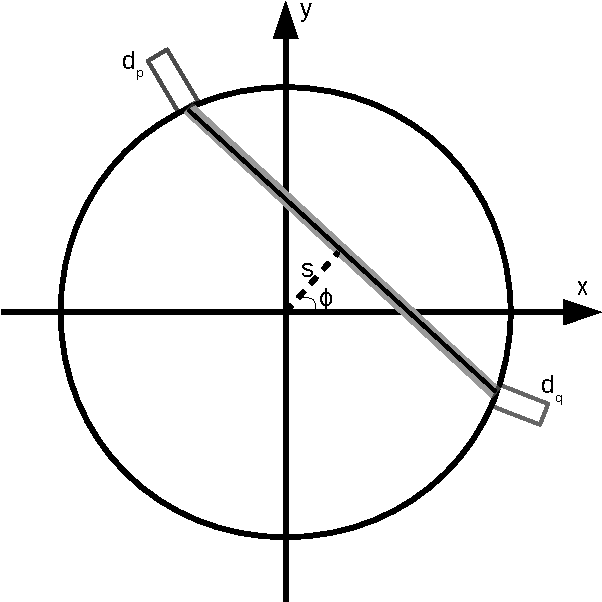
\includegraphics[width=0.6\linewidth]{./Figures/PET_det-crop.pdf}
	\caption{Depiction of a circular \ac{PET} detector with detectors $d_p$ and $d_q$ connected with a \ac{LOR} indicated in gray.}
	\label{fig:2dpet}
\end{figure}

 The number of detected coincidence events is related to the \ac{LOR} ($L_{d_{p},d_{q}}$) connecting the centers of detectors $d_p$ and $d_q$ through a sensitivity function $\psi(\vec{r}=(x,y,z))$. It is a Poisson variable whose mean can be written as:

\begin{equation}\label{eq:analy}
\left\langle p_{d_{p},d_{q}}\right\rangle=\tau \int_{\mathrm{FOV}} d \vec{r} f(\vec{r}) \psi_{d_{p}, d_{q}}(\vec{r})
\end{equation}

where $f(\vec{r})$ denotes tracer concentration and $\tau$ is the acquisition time. The tracer concentration is assumed to be contained within the \ac{FOV}. The reconstruction task can be summarized as estimating tracer concentration $f$, given measured data $p_{d_{p},d_{q}}$, $(d_{p},d_{q})=1\dots N_{LOR}$. The above linear model is typically used by analytical algorithms. The measurement data is assumed to have been corrected for non-linear effects like scatter and random coincidences. Another approximation is that $\psi(\vec{r})=0$, except when $r\in L_{d_{p},d_{q}} $. The measured data are therefore modeled as line integrals of tracer distribution ($f$): 

\begin{equation}
\label{eq:line}
\left\langle p_{d_{p}, d_{q}}\right\rangle=\int_{L_{d_{p}, d_{q}}} d \vec{r} f(\vec{r})
\end{equation}

The coincidences from the detector are typically rearranged either in listmode or sinogram format. List mode data is a sequential recording of coincidence events. Time and energy of each detected photon can also be recorded. It has special significance in time of flight imaging for \ac{PET}. Most analytical reconstruction algorithms on the other hand are tailor made for sinogram data format. Fig~\ref{fig:2dpet}, represents a trans-axial slice of a \ac{PET} scanner. One can model 2-D sinogram model with this representation. The variables $s$ and $\phi$ are utilized to relate the \ac{LOR} to the Cartesian co-ordinates $(x,y)$. The radial variable $s$ is the distance between the center of the detector ring and the \ac{LOR}, while angular variable ($\phi$) gives the orientation of the \ac{LOR}. 
For a co-ordinate $t$ along the line, Eq~\ref{eq:line} now becomes:
\begin{equation}\label{eq:line_sino}
\begin{array}{c}
p\left(s, \phi\right)=\int_{-\infty}^{\infty} d t f(x= s \cos\phi +t \sin \phi, 
\left.y=s \sin \phi + t \cos \phi\right)
\end{array}
\end{equation}

Through the line integral approximation and keeping in context the corrected \ac{PET} data, $p_{d_{a},d_{b}}\approx p(s,\phi)$. The function that maps the tracer distribution onto the line integrals is called as the x-ray transform. It is equivalent to the 2D version of the Radon transform. 

\section{CT}
% Write a paragraph on CT imaging

\ac{CT} imaging is a form of transmission tomography. The high resolution images obtained from \ac{CT} scans have many applications. They are extensively used in diagnosis of muscle, tissue and bone disorders. They serve a guide for surgery planning and also to pin-point exact location of tumors. In emergency situations like a road accident, \ac{CT} scan is utilized to check for internal bleeding. However, the radiation passed through the patient has been a topic of constant debate in this imaging modality. Research in recent times has been focusing on methodologies to reduce radiation while keeping the image quality intact. 


A typical \ac{CT} imaging setup consists of a X-ray source, the object to be imaged and detectors to measure the extent of attenuation experienced by the X-rays. When X-rays are passed through an object they suffer attenuation due to scatter and absorption. Scattering occurs when a X-ray photon dislodges an electron by transferring a part of it's energy. This phenomenon also called Compton scatter is depicted in Fig~\ref{fig:com}. 
\begin{figure}[!htbp]
	\centering
	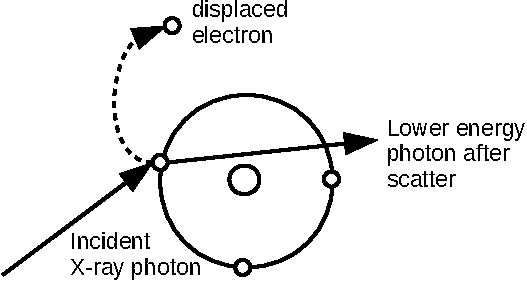
\includegraphics[width=0.7\linewidth]{./Figures/compton-crop.pdf}
	\caption{Depiction of Compton scatter}
	\label{fig:com}
\end{figure}

Complete absorption happens through photo-electric effect where the entire energy of the x-ray photon is transferred to the electron. The difference is seen in Fig~\ref{fig:photo}, where the incident photon disappears after scatter. 

\begin{figure}[!htbp]
	\centering
	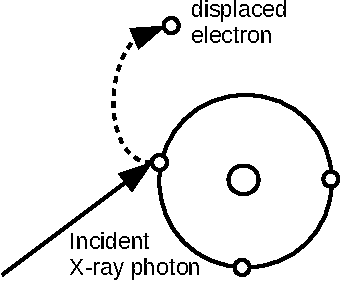
\includegraphics[width=0.5\linewidth]{./Figures/photo-crop.pdf}
	\caption{Depiction of Photo-electric effect}
	\label{fig:photo}
\end{figure}


Different materials exhibit different absorption properties hence have unique linear attenuation co-efficient. Let the intensities of incident x-ray and the one after absorption be $I_{0}$ and $I_{a}$ respectively. From Beer-Lambert's law, we have:

\begin{equation}\label{eq:BL}
I_{a} = I_{0} \cdot \exp (-p) 
\end{equation}

where p is the line integral of attenuation coefficients along the path of the x-ray photons. Similar to \ref{eq:line}, measured data in \ac{CT} can be modeled with line integrals $p$:
\begin{equation}\label{eq:l_CT}
p =\ln \frac{I_{a}}{I_{0}} 
\end{equation}
The material specific property of attenuation ($\mu$) varies with the energy of the incoming X-ray. It reduces with the increase in energy of the X-ray. A cross-sectional \ac{CT} image consists of 

Over the years many imaging geometries have been developed to maximize detector efficiency and obtain better image quality. The first generation of \ac{CT} scanners consisted of X-ray beam source and a small detector that rotated and linearly translated around the patient. It had much longer scanning time compared to modern \ac{CT} scanners. The second generation setup consisted of fan-beam source with an array of detectors. The motion was similar to that of the first generation. The third generation fan beam geometry is depicted in Fig~\ref{fig:xgeo}, the motion was restricted to rotation of the source-detector setup. The fourth generation consisted of stationary circular array of detectors similar to \ac{PET} with a rotating source. 
\begin{figure}[!htbp]
	\centering
	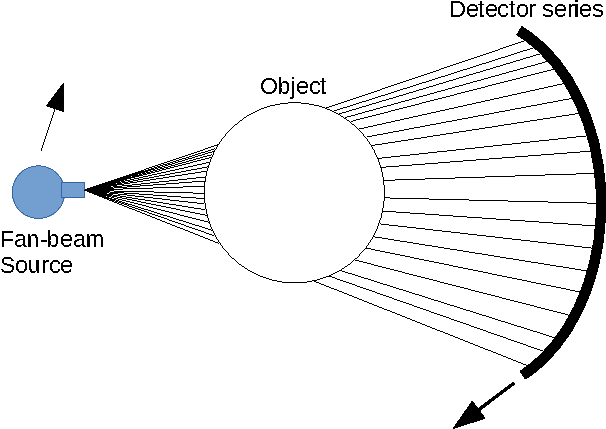
\includegraphics[width=0.6\linewidth]{./Figures/x_ray_geo-crop.pdf}
	\caption{Fan-beam geometry: the source and the detector rotate around the object}
	\label{fig:xgeo}
\end{figure}

\begin{figure}[!htbp]
	\centering
	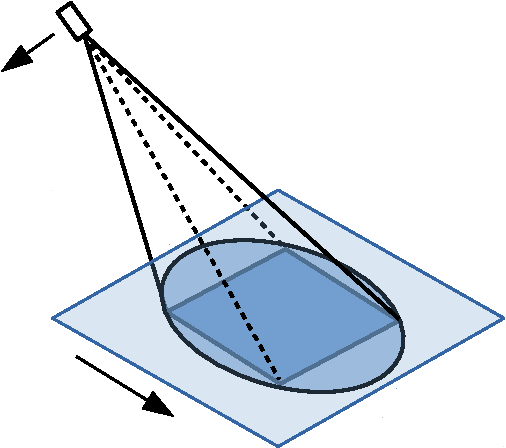
\includegraphics[width=0.6\linewidth]{./Figures/cbct-crop.pdf}
	\caption{Cone-beam geometry: the source rotates around the patient while the bed is translated creating a helical scan.}
	\label{fig:cbct}
\end{figure}
A representation of a modern helical cone beam scanner is shown in Fig~\ref{fig:cbct}. The cone-beam source is rotated around the patient while the bed translates linearly resulting in a helical orbit. The detector is a 2D array of crystals making it more efficient and faster for data acquisition.

\section{Analytic Reconstruction}

The starting point of analytic reconstruction is the central slice theorem. It states that 2D Fourier transform of the image ($f$) is related to the 1D Fourier transform of the x-ray transform as follows:

\begin{equation}
P(v, \phi)=f\left(v_{x}=v \cos \phi, v_{y}=v \sin \phi\right)
\end{equation} 

where

\begin{equation}
P(v, \phi)=(\mathcal{F} p)(v, \phi)=\int_{\mathbb{R}} d s p(s, \phi) \exp (-2 \pi i s v)
\end{equation}

and $v$ is the frequency variable associated with $s$. In the context of tomographic image reconstruction this theorem has the following implication: given the measurement data for all projection angles $\phi \in [0,\pi]$, the radial line sweeps all the frequencies hence making it possible to compute $f(v_{x},v_{y})$ for $(v_{x},v_{y})\in \mathbb{R}^2$. The image $f$ can then be estimated by finding the inverse 2D Fourier transform. 

\subsubsection{FBP}

One of the most used reconstruction algorithms across modalities is the filtered back-projection algorithm. The version with continuous sampling is written as follows:


\begin{equation}
\begin{array}{l}
f(x, y)=\left(X^{*} p^{F}\right)(x, y)= 
\int_{0}^{\pi} d \phi p^{F}(s=x \cos \phi+y \sin \phi, \phi)
\end{array}
\end{equation}


where filtered projections $p^{F}$ are given by

\begin{equation}
p^{F}(s, \phi)=\int_{-R_{F}}^{R_{F}} d s^{\prime} p\left(s^{\prime}, \phi\right) h\left(s-s^{\prime}\right)
\end{equation}


and $h$ is the ramp filter given by

\begin{equation}
h(s)=\int_{-\infty}^{\infty} d v|v| \exp (2 \pi i s v)
\end{equation}



The function mapping from $p^{F}$ to $\lambda$ is the back-projection operator. 
In reality discrete sampling is required to accurately model the acquisition process. The discrete implementation of the \ac{FBP} can be written as follows:

\begin{equation}\label{eq:FBP}
\boldx(i,j) = \frac{\pi}{N_\phi}\sum_{l=0}^{N_\phi-1}\boldy_f(s=i\cos\phi_l+j\sin\phi_l,\phi_l)
\end{equation}

where $x$ is the image for a set of pixels $(i,j)$, $\boldy_f$ are the filtered projections obtained by filtering the projections, expressed in terms of radial variable $s$ and projection angle $\phi$, and $N_\phi$ number of projection angles. The above equation is the approximation of backprojection by a discrete quadrature. 




\section{Model-Based Image Reconstruction (MBIR)}

Analytical methods are faster to implement and practical in a clinical setting but they are vulnerable to noise. The assumptions made in analytical formations are that the measurements are continuous and the solutions are of integral formulation. Sampling is done to the data a posteriori. They are also highly susceptible to system geometry. Since the 80's, \ac{MBIR} techniques (\cite{Shepp1982,fessler2000statistical}) became the standard approach. As they model the stochasticity of the system, they are more robust to noise as compared with \ac{FBP}, and can be completed with a penalty term for additional control over the noise (\cite{depierro1995}). They also incorporate corrections for scatter and are independent of detector geometry.

\subsection{Data Model for PET}
The starting point of any model-based method is the data model. The measurement $\boldy$ is a random vector modeling the number of detection (photon counting) at each of the $n$ detector bins, and follows a Poisson distribution with independent entries:
\begin{equation}\label{eq:poisson}
\boldy \sim \mathrm{Poisson}(\boldybar(\boldx))
\end{equation}    
where $\boldybar(\boldx) \in \bbR^n$ is the expected number of counts (noiseless), which is a function of the image $\boldx$. 

The expected number of counts is
\begin{equation}\label{eq:PET}
\boldybar(\boldlambda) = \boldA \boldlambda
\end{equation}
where $\boldA \in \bbR^{n\times m}$ is a system matrix such that each entry $[\boldA]_{i,j}$ represents the probability that a photon pair emitted from voxel $j$. Image reconstruction is achieved by finding a suitable image $\boldxhat = \boldlambdahat$ that approximately solves 
\begin{equation}\label{eq:pb1solve}
\boldy = \boldybar(\boldx) \, .
\end{equation} 


\subsection{Data Model for CT}
Let an image be represented by $\boldx \in \bbR^m$ and the scanner measurement by $\boldb \in \bbR^n$ where $m$ is the number of voxels and $n$ is the number of measurements. In \ac{2D} \ac{CT} imaging $n$ depends on the number of detectors $N_\mathrm{d}$ and the number of angles $N_\mathrm{a}$. The task of medical image reconstruction corresponds to finding a mapping from $\boldb$ to $\boldx$. The measurement $\boldb$ is a random vector modeling the number of detection (photon counting) at each of the $n$ detector bins, and follows a Poisson distribution with independent entries, i.e.,
\begin{equation}\label{eq:pCT}
\boldb \sim \mathrm{Poisson}(\boldbbar(\boldx))
\end{equation}    
where, $\boldb  =  [b_1(\boldx),\dots,b_n(\boldx)]\transp\in \bbR^n$ and $\boldbbar(\boldx)  =  [\bbar_1(\boldx),\dots,\bbar_n(\boldx)]\transp\in \bbR^n$ is the expected number of counts (noiseless), which is a function of the image $\boldx$. 

The image $\boldx\in\mathbb{R}^m$ is a vectorized input image (also referred to as attenuation) representing the measure of X-rays absorbed or scattered as they pass through the patient. In a monochromatic setting, the expected number of counts $\boldbbar(\boldx)$  is given by the Beer-Lambert law, i.e.,
\begin{equation}\label{eq:CT}
\bbar_i(\boldx) = I \cdot \exp (-[\boldA \boldx]_i) \quad \forall i=1,\dots,n 
\end{equation}
where, $I$ is the intensity and $\boldA \in \bbR^{n\times m}$ is a system matrix such that each entry $[\boldA]_{i,j}$ represents the contribution of the $j$-th image voxel to the $i$-th detector. Given the raw projections $\boldbbar$, we take the logarithm as follows
\begin{equation}
y_i = \log\left(\frac{I}{b_i}\right) \quad \forall i=1,\dots,n   
\end{equation}
where we assumed that the intensity $I$ is sufficiently high so that $b_i>0$ for all $i$. Image reconstruction is based on finding a suitable image $\boldxhat$ that approximately solves 
\begin{equation}\label{eq:pb2solve}
\boldy = \boldA \boldxhat 
\end{equation} 

where $\boldy  =  [y_1,\dots,y_n]\transp\in \bbR^m$. The reconstruction can also be achieved with more sophisticated iterative techniques that account for the stochastic properties of the measurement \eqref{eq:poisson} \cite{nuyts1998iterative,Elbakri2002}.

In a sparse-view setting, the number of rotation angles of the detector is decreased in order to reduce the radiation passing through the patient. This implies a reduction in the number of projection angles in the measurement $\boldy$.

\subsection{Maximum Likelihood Expectation Maximization (MLEM)}
The most famous model based method for \ac{PET} image reconstruction is the \ac{MLEM} algorithm. The cost function for \ac{MLEM} is based on Poisson likelihood given as follows:
\begin{equation}\label{eq:poisson_like}
\operatorname{Pr}\{\boldybar \mid \boldx\}=\prod_{j=1}^{N_{L o R}} \exp \left(-\left\langle y_{j}\right\rangle\right)\left\langle y_{j}\right\rangle^{y_{j}} / y_{j} !
\end{equation}

Putting \ref{eq:PET} in \ref{eq:poisson_like}, taking log and dropping terms that do not depend on unknown image $x$ we get the cost function for \ac{MLEM},

\begin{equation}
Q(\boldxbar, \boldybar)=\sum_{j=1}^{N_{L O R}}\left\{-\sum_{i=1}^{m} \boldA_{j, i} x_{i}+y_{j} \log \left(\sum_{i=1}^{m} \boldA_{j, i} x_{i}\right)\right\}
\end{equation}
where $Q$ is the cost function and the definition of other variables is consistent from above. As long as the matrix $\boldA$ is singular, the above cost function remains convex and results in a unique image. 
The update step to map from the current estimate $x^{n}$ to the next estimate $x^{n+1}$ can be written as follows:

\begin{equation}\label{eq:mlem}
\boldx_{i}^{n+1}=x_{i}^{n} \frac{1}{\sum_{j^{\prime}=1}^{N_{L o R}} \boldA_{j^{\prime}, i}} \sum_{j=1}^{N_{L O R}} \boldA_{j, i} \frac{y_{j}}{\sum_{i^{\prime}=1}^{m} \boldA_{j, i^{\prime}} x_{i^{\prime}}^{n}} \quad i=1, \ldots, m
\end{equation}

The initial estimate $x_i^{1}$, $i=1, \ldots, m$ typically follows a uniform distribution. The denominator with sum over index $i^{\prime}$ is the forward projection operation. Hence it estimates the measured data for the current image estimate. The numerator with sum over index $j$ is the back projection over the ratio of measured and estimated data. The \ac{MLEM} algorithm does not include a prior and it converges to the image that best fits the data. This estimate has inherent instabilities as the fitting is done closely to the noisy measured data. Contrary to \ac{FBP}, data corrections in \ac{MLEM} can be added to the cost function. Attenuation correction can be introduced as a multiplicative factor while scatter and randoms are added to the cost function as follows:

\begin{equation}
\begin{array}{l}
\boldx_{i}^{n+1}=x_{i}^{n} \frac{1}{\sum_{j^{\prime}=1}^{N_{L O R}} \boldA_{j^{\prime}, i} / \alpha_{j^{\prime}}} \sum_{j=1}^{N_{L o R}} \boldA_{j, i} \frac{y_{j}+2 \bar{r}_{j}+\bar{s}_{j}}{\sum_{i^{\prime}=1}^{m} \boldA_{j, i^{\prime}} x_{i^{\prime}}^{n}+\alpha_{j}\left(2 \bar{r}_{j}+\bar{s}_{j}\right)} \\
i=1, \ldots, m
\end{array}
\end{equation}

where $y_j$ are measured data corrected for random and scatter, $\alpha_{j}$ is the factor for attenuation correction, $\bar{r}_{j}$ and $\bar{s}_{j}$ are estimates for random and scatter background in \ac{LOR} $j$. 



\subsection{Ordered Subsets Expectation Maximization (OSEM)}

The \ac{OSEM} algorithm is a modification of the \ac{MLEM} algorithm which made it computationally practical for implementation in clinical setting. The \ac{LOR} data is divided into $\bm{S}$ disjoint subsets: $J_{1}, \cdots, J_{S} \subset\left[1, \cdots, N_{\text {LOR }}\right]$. Each of the parallel projection is assigned to a unique subset: $c, c+S, c+2S, \cdots, \leq N_{\phi}$ to the subset $J_{c+1}$. \ac{MLEM} (Eqn~\ref{eq:mlem}) is applied to each of the subsets individually in an orderly fashion. Subset $J_{N\bmod S}$ is used at iteration $N$:

\begin{equation}
\begin{array}{l}
\boldx_{i}^{N+1}=\boldx_{i}^{N} \frac{1}{\sum_{j^{\prime} \in J_{N \bmod S}} \boldA_{j^{\prime}, i}} \sum_{j \in J_{N \bmod S}} \boldA_{j, i} \frac{y_{j}}{\sum_{i^{\prime}=1}^{m} \boldA_{j, i^{\prime}} \boldx_{i^{\prime}}^{N}} \\
i=1, \ldots, m
\end{array}
\end{equation}  

%-----------------------------------
%	SUBSECTION 2
%-----------------------------------



\subsection{Weighted Least Squares (WLS)}

One of the most common iterative techniques for \ac{CT} image reconstruction is the \ac{WLS} method, the image $\xhat$ is estimated by minimizing the following:

\begin{equation}
\hat{x}=\underset{x \succeq 0}{\arg \min } \frac{1}{2}\|y-A x\|_{W}^{2}
\end{equation}

where $W=\operatorname{diag}\left\{w_{i}\right\}$ is the diagonal weighting matrix that constitutes for the variance of each ray and $\|z\|_{W}^{2}=z^{\prime} W z$. Despite the statistical weighting, due to the noise in measurements and ill-conditioned problem of image reconstruction the image estimate will still be noisy. 

\subsection{Penalized MBIR}
An improvement to the above mentioned \ac{MBIR} algorithms can be brought by finding a balance between the desired a priori characteristics of the image and the data fitting. This balance is realized through a regularized cost function.

\subsubsection{Absolute Difference}
One such form of regularization is introduced through an edge preserving regularizer that penalized the differences between neighboring voxels:

\begin{equation}
R(x)=\sum_{j=1}^{n_{\mathrm{p}}} \sum_{k \in \mathcal{N}_{j}} \psi_{j k}\left(x_{j}-x_{k}\right)
\end{equation}

where $R(x)$ is the regularization term, that enforces piece-wise smoothness on the image and $\beta$ the regularization parameter. $\psi$ is a potential function that controls the penalization of differences in the neighboring voxels. Adding the penalty term in the cost function of \ac{WLS} we get:
 
\begin{equation}
\hat{x}=\underset{x \succeq 0}{\arg \min } \Psi(x), \quad \Psi(x) \triangleq \frac{1}{2}\|y-A x\|_{W}^{2}+\beta R(x)
\end{equation} 
   

where $N_j$ are the set of neighboring indices of the $j^\mathrm{th}$ voxel. 

\subsubsection{Total Variation (TV)}
Complex image reconstruction problems like sparse-view \ac{CT} are under-determined due to the limited number of projection data available for reconstruction. In such a scenario stronger forms of regularization like \ac{TV} are utilized. Consider a 2D digital image $x[p,q]$, discrete form of \ac{TV} can be written as:

\begin{equation}
\sum_{p} \sum_{p}|x[p, q]-x[p-1, q]|+|x[p, q]-x[p, q-1]|
\end{equation}    

This is an an-isotropic version of \ac{TV} regularization. Images reconstructed with \ac{TV}, sometimes have inexplicable artifacts due to the fact that the absolute value potential is not differentiable at $0$. 

